\documentclass{article}

% Language setting
% Replace `English' with e.g. `Spanish' to change the document language
\usepackage[english]{babel}
\usepackage{ctex}

% Set page size and margins
% Replace `letter paper' with`a4paper' for UK/EU standard size
\usepackage[a4paper,top=1.5cm,bottom=1.5cm,left=2cm,right=2cm,marginparwidth=1.75cm]{geometry}

% Useful packages
\usepackage{amsmath}
\usepackage{amssymb}
% 引入{amssymb}包,避免输入\nexists(存在否定)这个符号时 报未定义符号的错误
\usepackage{graphicx}
\usepackage{listings}
\usepackage[ruled]{algorithm2e}
\usepackage[colorlinks=true, allcolors=blue]{hyperref}
\usepackage{algpseudocode}
\usepackage{ dsfont }
% \usepackage{algorithm}

\SetKwProg{Function}{function}{:}{end}

% TODO 个人信息参数全局变量
% -------------- define personal variables begin --------------
\newcommand\myCollege{}
\newcommand\myId{22373058}
\newcommand\myName{胡健}
\newcommand\myHomeworkId{1}
% --------------  define personal variables end  --------------

\title{\heiti \myCollege《算法设计与分析》第\myHomeworkId 次作业} % 文章标题
\author{\myCollege \quad \myId \quad \myName} % 作者信息

\begin{document}
\maketitle

\section{请给出 T(n) 尽可能紧凑的渐进上界并予以说明 (每小题 3 分,共 21 分)} % TODO 作业题目1名字

\subsection{} % TODO 作业题目1.1名字

% TODO 大括号样例

$$
\left\{
\begin{array}{l}
T(n)=1\ ,\ n=1\\
T(n)=T(n-1)+n\ ,\ if\ n>1
\end{array}
\right.
$$

解:

\begin{align*}
T(n)&=T(n-1)+n\\
    &=T(n-2)+n+(n-1)\\
    &=T(n-3)+n+(n-1)+(n-2)\\
    &=\cdots \\
    &=n+(n-1)+(n-2)+...+2+1\\
    &=\frac{1}{2}n(n+1)\\
    &=O(n^2)
\end{align*}


\quad\quad\quad\quad 由此可知,原式渐进上界为$O(n^2)$。


\subsection{} % TODO 作业题目1.2名字

$$
\left\{
\begin{array}{l}
T(1) = 1, T(2) = 1\\
T(n) = T(n-2) +1,\ if \ n>2
\end{array}
\right.
$$

解:

\begin{align*}
T(n)&=T(n-2)+1\\
    &=T(n-4)+1+1\\
    &=\cdots \\
    &=1+\cdots + 1 + T(2-n\%2)\\
    &=\lceil \frac{n}{2} \rceil\\
    &=O(n)
\end{align*}



\subsection{}

$$
\left\{
\begin{array}{l}
T(1) = 1\\
T (n) = 4T (n/2) + n,\ if\ n > 1
\end{array}
\right.
$$

解:

\quad\quad\quad\quad 由主定理法

\begin{align*}
    &\text{if}\  T(n) = a T(\frac{n}{b}) + O(n^d),\\
    &则T(n) = 
    \begin{cases}
        O(n^d), & \textbf{if } d > \log_ba\\
        O(n^d\log n),& \textbf{if } d = \log_ba\\
        O(n^{\log_ba}), & \textbf{if } d < \log_ba
    \end{cases}
\end{align*}

\quad\quad\quad\quad 这里有$a = 4, b = 2, d = 1$

\quad\quad\quad\quad 那么$d < log_b a = 2$

\quad\quad\quad\quad 所以$T(n) = O(n^d) = O(n^2)$



\subsection{}

$$
\left\{
\begin{array}{l}
T(1) = 1\\
T(n) = 8T(n/2) +n^3\ ,\ if \ n>1
\end{array}
\right.
$$


解:

\quad\quad\quad\quad 由主定理法

\begin{align*}
    &\text{if}\  T(n) = a T(\frac{n}{b}) + O(n^d),\\
    &则T(n) = 
    \begin{cases}
        O(n^d), & \textbf{if } d > \log_ba\\
        O(n^d\log n),& \textbf{if } d = \log_ba\\
        O(n^{\log_ba}), & \textbf{if } d < \log_ba
    \end{cases}
\end{align*}

\quad\quad\quad\quad 这里有$a = 8, b = 2, d = 3$

\quad\quad\quad\quad 那么$d = log_b a = 3$

\quad\quad\quad\quad 所以$T(n) = O(n^d) = O(n^3logn)$

% \newpage

\subsection{}

$$
\left\{
\begin{array}{l}
T(1) = 1, T(2) = 1\\
T(n) = 2T(n/3) + n^2\ ,\ if \ n>2
\end{array}
\right.
$$


解:

\quad\quad\quad\quad 由主定理法

\begin{align*}
    &\text{if}\  T(n) = a T(\frac{n}{b}) + O(n^d),\\
    &则T(n) = 
    \begin{cases}
        O(n^d), & \textbf{if } d > \log_ba\\
        O(n^d\log n),& \textbf{if } d = \log_ba\\
        O(n^{\log_ba}), & \textbf{if } d < \log_ba
    \end{cases}
\end{align*}

\quad\quad\quad\quad 这里有$a = 2, b = 3, d = 2$

\quad\quad\quad\quad 那么$d = 2 > \log_b a $

\quad\quad\quad\quad 所以$T(n) = O(n^d) = O(n^2)$

\subsection{}

$$
\left\{
\begin{array}{l}
T(1) = 1\\
T (n) = T (n/2) + \log n\ ,\ if \ n>1
\end{array}
\right.
$$

解:

\begin{align*}
T(n)&=T(n/2) + \log n \\
    &=T(n/4) + \log \frac{n}{2} + \log n \\
    &=\cdots\\
    &=T(1) + \log 2 + \log 4 + \cdots + \log \frac{n}{2} + \log n\\
    &=1+\log (\Pi_{i = 1}^n 2^i)\\
    &=1+\log (\sqrt{\Pi_{i = 1}^{\log n} 2^i * 2^{\log n - i})})\\
    &=1+\log (\sqrt{\Pi_{i = 1}^{\log n} 2^{\log n})})\\
    &=1+\frac{1}{2}\log ( 2^{{\log n} \times \log n}))\\
    &=1+\frac{1}{2} \log n \times \log n\\
    &=O(\log^2 n)
\end{align*}

\quad\quad\quad\quad 由此可知,原式渐进上界为$O(\log^2 n)$。

% \newpage

\subsection{}

$$
\left\{
\begin{array}{l}
T(1) = 1\\
T(n) = T(n-1) +2^n\ ,\ if \ n>1
\end{array}
\right.
$$

解:

\begin{align*}
T(n)&=T(n-1) + 2^n \\
    &=T(n-2) + 2^{n-1} + 2^n \\
    &=\cdots\\
    &=T(1) + 2^2 + 2^3 + \cdots + 2^n\\
    &=2^{n+1} - 3\\
    &=O(2^n)
\end{align*}

\quad\quad\quad\quad 由此可知,原式渐进上界为$O(2^n)$。

% \newpage

\section{游戏获奖问题 (19 分)} % TODO 作业题目2名字

% TODO 作业题目2描述

在一场射击比赛中,有 $n$ 名选手参加比赛,每名选手的得分都不同,记为 $s[1...n]$,其中第 $i$名选手的得分为$ s[i]$,且对于任意的$ i\ne j $有 $s[i]  \ne s[j]$。按照比赛规则,分数排名为前$ \lfloor n/3\rfloor $的选手可以获得与其得分相等的奖金(包括第 ⌊n/3⌋ 名)。

例如,当有 6 名选手参加比赛,得分为 s = [100, 50, 90, 60, 65, 80] 时,排名位于前 ⌊6/3⌋ = 2的选手得分为 100, 90,则主办方应该发放奖金 190 元。

请你设计一个算法,计算这次比赛主办方一共要发放多少奖金。请描述算法的核心思想,给
出算法伪代码并分析其对应的时间复杂度。

\subsection{题目分析与核心思想} % TODO 作业题目2分析

本题最直观的一个思路是对数组进行排序,然后取前$\lfloor \frac{n}{3}\rfloor$个元素求和即可。

\begin{enumerate}
    \item 对于排序,使用基于比较的排序,如\textbf{归并排序},那么时间复杂度为$O(n\log n)$
    \item 这里可以认为选手得分均为非负整数,那么可以使用\textbf{桶排序(计数排序)},然后取最大的$\lfloor \frac{n}{3}\rfloor$个元素求和,那么时间复杂度为$O(n+k)$,其中k为选手得分的最大值
\end{enumerate}

然后考虑的一个点是,排序是把数组的每个元素的序都确定了,如果只是取出最大的$\lfloor \frac{n}{3}\rfloor$个元素,实际上不需要全部排序。那么就有使用类似快速排序的\textbf{快速选择}的算法,最好时间复杂度和期望时间复杂度均为$O(n)$,最坏时间复杂度为$O(n^2)$。

\subsection{算法与伪代码} % 作业题目2算法与伪代码

\subsubsection{基于排序算法}

% TODO 伪代码模板

\begin{algorithm}[H]

\caption{基于归并排序处理游戏获奖问题}
\LinesNumbered
\KwIn{正整数$n$,为数组长度,每名选手的得分数组:$A[1...n]$}
\KwOut{一个整数Ans,表示主办方发放的奖金}

\Function{$main(n,A)$}{
    $\text{MergeSort}(A, 1, n)$\\
    $Ans \leftarrow 0 $\\
    \For {$i \leftarrow 1 \ to \ \lfloor \frac{n}{3} \rfloor$} {
        $Ans += A[i]$
    }
    \Return{$Ans$}
}

\Function{$MergeSort(A,left,right$)}{
    \If{$left \ge right$}{
        \Return{$A[left..right]$}
    }
    $mid \leftarrow \lfloor \frac{left+right}{2} \rfloor$\\
    $\text{MergeSort}(A, left, mid)$\\
    $\text{MergeSort}(A,mid+1, right)$\\
    $\text{Merge}(A,left, mid, right)$\\
    \Return{A[left..right]}\\
}
\Function{$Merge(A, left, mid, right)$}{
    $A'[left, right] \leftarrow A[left, right]$\\
    $i\leftarrow left, j \leftarrow mid+1,k\leftarrow 0$\\
    \While{$i\le mid\ and\ j \le right$}{
        \If{$A'[i] \le A'[j]$}{
            $A[left+k] \leftarrow A'[i]$\\
            $k\leftarrow k+1, i\leftarrow i+1$
        }
        \Else{
            $A[left+k] \leftarrow A'[j]$\\
            $k\leftarrow k+1, j\leftarrow j+1$
        }
    }
    \If{$i \le mid$}{
        $A[left+k..right] \leftarrow A'[i..mid]$
    }
    \Else{
        $A[left+k..right] \leftarrow A'[j..right]$
    }
    \Return{A[left..right]}
}

\end{algorithm}

\begin{algorithm}[H]

\caption{基于计数排序处理游戏获奖问题}
\LinesNumbered
\KwIn{正整数$n$,为数组长度,每名选手的得分数组:$A[1...n]$}
\KwOut{一个整数Ans,表示主办方发放的奖金}

\Function{$main(n,A)$}{
    $max \leftarrow 0$
    \For{$i \leftarrow 1 \ to \ n$}{
        \If{$max < A[i]$}{
            $max = A[i]$
        }
    }
    $\text{CountingSort}(A, n, max)$\\
    $Ans \leftarrow 0 $\\
    \For {$i \leftarrow 1 \ to \ \lfloor \frac{n}{3} \rfloor$} {
        $Ans += A[i]$
    }
    \Return{$Ans$}
}

\Function{$CountingSort(A,n,max$)}{
    $T[0..max] \leftarrow [0] * (max+1)$\\
    \For{$i \leftarrow 1 \ to \ n$}{
        $T[A[i]] \leftarrow T[A[i]] + 1$
    }
    $j\leftarrow 0$\\
    \For{$i \leftarrow 0 \ to \ max$} {
        \While{$T[i] > 0$}{
            $A[j] \leftarrow i$\\
            $T[i] \leftarrow T[i] - 1$\\
            $j\leftarrow j+1$
        }
        \If{$j = n -1$}{
            \textbf{Break}
        }
    }
}

\end{algorithm}

\subsubsection{基于快速选择算法}

\begin{algorithm}[H]

\caption{基于快速选择算法处理游戏获奖问题}
\LinesNumbered
\KwIn{正整数$n$,为数组长度,每名选手的得分数组:$A[1...n]$}
\KwOut{一个整数Ans,表示主办方发放的奖金}

\Function{$main(n,A)$}{
    $price\leftarrow \text{RandomizedSelection}(A, 1, n, \lfloor \frac{n}{3} \rfloor)$\\
    $Ans \leftarrow 0 $\\
    \For {$i \leftarrow 1 \ to \ n$} {
        \If{$A[i] \ge price$}{
            $Ans \leftarrow Ans + A[i]$
        }
    }
    \Return{$Ans$}
}
\Function{$RandomizedSelection(A, p, r,k)$}{
    $q\leftarrow \text{RandomizedPartition}(A,p,r)$\\
    \If{$k = (q-p+1)$}{
        $x\leftarrow A[q]$
    }
    \If{$k < (q-p+1)$}{
        $x \leftarrow \text{RandomizedSelection}(A, p, q-1,k)$
    }
    \If{$k > (q-p+1)$}{
        $x \leftarrow \text{RandomizedSelection}(A, q+1, r,k-(q-p+1)$
    }
    \Return{$x$}
}
\Function{$RandomizedPartition(A,p,r)$}{
    $s=\text{Random}(p,r)$ \Comment{随机选择主元}\\
    $\text{exchange}\ A[s]\ \text{with}\ A[r]$\\
    $x\leftarrow A[r]$\\
    $i\leftarrow p-1$\\
    \For{$j\leftarrow p \ to \ r-1$}{
        \If{$A[j] \ge x$}{
            $\text{exchange}\ A[i+1]\ \text{with}\ A[j]$\\
            $i\leftarrow i+1$
        }
    }
    $\text{exchange}\ A[i+1]\ \text{with}\ A[r]$\\
    $q\leftarrow i+1$\\
    \Return{$q$}
}
\end{algorithm}

\subsection{时间复杂度分析}

基于\textbf{归并排序}处理游戏获奖问题时,算法主要分为排序阶段与求和阶段,排序阶段的时间复杂度递推式为
$T(n)=T(\frac{n}{2}) + O(n)$,由主定理可求得时间复杂度为$O(n\log n)$,求和阶段的时间复杂度为$O(n)$,因此算法的总时间复杂度为$O(n \log n)$

基于\textbf{计数排序}处理游戏获奖问题时,算法主要分为排序阶段与求和阶段,排序阶段为主要包括遍历原数组和遍历长度为数组元素最大值的数组两个部分,时间复杂度为$O(n+k)$,其中k为数组元素的最大值,求和阶段的时间复杂度为$O(n)$,因此算法的总时间复杂度为$O(n +k)$

基于\textbf{快速选择}算法处理游戏获奖问题时,算法的主要分为固定位置次序选择部分和遍历数组取大于第$\lfloor \frac{n}{3}\rfloor$的元素的所有元素,固定位置次序选择时调用了随机化的固定位置划分,最优解为第一次即找出了第$\lfloor \frac{n}{3}\rfloor$的元素,时间复杂度为$O(n)$,最坏情况为$T(n) = O(n) + O(n-1)+\cdots O(1) = \sum_{i=1}^n i = O(n^2)$,期望复杂度为$O(n)$。之后遍历的时间复杂度为$O(n)$,因此最终的期望时间复杂度为$O(n)$

下面证明基于快速选择期望复杂度为$O(n)$

随机选择主元,共$n$种情况(假设元素互不相同):
$$
T(n) \le
\begin{cases}
max{T(0), T(n-1)} + O(n)= T(n-1) + O(n)\\    
max{T(1), T(n-2)} + O(n)= T(n-2) + O(n)\\    
max{T(2), T(n-3)} + O(n)= T(n-3) + O(n)\\    
\cdots \\
max{T(n-1), T(0)} + O(n)= T(n-1) + O(n)\\    
\end{cases}
$$

每种情况出现的概率均为$\frac{1}{n}$,每个$T(i)出现2次,i\ge \lfloor \frac{n}{2} \rfloor$

期望时间:
\begin{align*}    
E[T(n)]&\le E[\frac{2}{n} \cdot \sum_{i=\lfloor \frac{n}{2} \rfloor}^{n-1} (T(i) + O(n))] \\
&\le\frac{2}{n} \cdot E[ \sum_{i=\lfloor \frac{n}{2} \rfloor}^{n-1} (T(i) + O(n))]\\
&=\frac{2}{n} \cdot  \sum_{i=\lfloor \frac{n}{2} \rfloor}^{n-1} E[(T(i))] + \frac{2}{n}\cdot  \sum_{i=\lfloor \frac{n}{2} \rfloor}^{n-1} O(n)\\
&=\frac{2}{n} \cdot  \sum_{i=\lfloor \frac{n}{2} \rfloor}^{n-1} E[(T(i))] + O(n)\\
\end{align*}

通过代入法分析期望可得,假设:$\forall i < n, E[T(i)] < c \cdot i$

那么代入有$E[T(n)]\le O(n) + \frac{2}{n} \sum_{i=\lfloor \frac{n}{2} \rfloor}^{n-1} c\cdot i\le O(n) + \frac{2}{n}\cdot c\cdot \frac{3}{8}n^2\le c \cdot n$

综上即证

% \newpage

\section{奇数因子和问题 (20 分)} % TODO 作业题目3名字

% TODO 作业题目3描述

定义 $od(i)$ 为整数 $i$ 的最大奇数因子,例如 $od(3) = 3,\ od(14) = 7$。


请你设计一个高效算法,计算一个整数区间$ [A, B] $内所有数的最大奇数因子和,即$\sum_{i \in [A,B]} od(i)$。请描述算法的核心思想,给出算法伪代码并分析其对应的时间复杂度。

例如,区间 [3, 9] 的计算结果为 3 + 1 + 5 + 3 + 7 + 1 + 9 = 29。

\subsection{题目分析与核心思想}

本题最直接的想法是直接暴力求解,对于每一个函数$od(n), n \in \mathds{Z}$,设$t = abs(n) = |n|$有
\begin{align*}
    &od(n) = od(t) = \begin{cases}
        t, & t\mod2 = 1\\
        \frac{t}{2}, & t\mod2=0
    \end{cases} 
\end{align*}

那么计算每个数$n$的$od(n)$的时间复杂度为$O(\log n)$,那么计算整数区间$[A,B]$的所有数的最大奇数因子和的时间复杂度为$(B-A)\log B$

通过观察函数的性质,我们发现可以将区间作为一个整体来进行考虑,于是有:

设所求整数区间$[A,B]$的所有数的最大奇数因子和为$S(A,B)$,这里我们发现有

\begin{align*}
    &S(A,B) = 
    \begin{cases}
     S(0,B) - S(0, A-1), & 0 < A \le B\\
     S(0,B) + S(A, 0) = S(0, B) + S(0, -A), & A \le 0 \le B\\
     S(A,0) - S(B+1, 0) = S(0, -A) - S(0, -B-1), & A \le B < 0 \\
    \end{cases}
\end{align*}

因此我们可以定义一个新的函数$f(n),n\in \mathds{Z}^*$表示整数区间$[0, n]$的所有数的最大奇数因子和。

那么就有

\begin{align*}
    &S(A,B) = 
    \begin{cases}
     f(B) - f(A-1), & 0 < A \le B\\
     f(B) + f(-A), & A \le 0 \le B\\
     f(-A) - f(-B-1), & A \le B < 0 \\
    \end{cases}
\end{align*}

因此所求的$S[A,B]$,只需计算函数$f$的相应的值即可。

易知$f(0) = 0, f(1) = 1$,对于$f(n), n > 1\ \wedge n  \in \mathds{Z}$,考虑如下递推式

\begin{align*}
    f(n)&=\sum_{i=0}^n od(i)\\
        &=(od(1) + od(3) + \cdots + od(2 \lceil \frac{n}{2} \rceil-1)) + (od(2) + od(4) + \cdots + od(2 \lfloor \frac{n}{2} \rfloor) \\
        &=\sum_{i=1}^{\lceil \frac{n}{2} \rceil} od(2i-1) +  \sum_{i=1}^{\lfloor \frac{n}{2} \rfloor} od(2i)\\
        &=\sum_{i=1}^{\lceil \frac{n}{2} \rceil} (2i-1) +  \sum_{i=1}^{\lfloor \frac{n}{2} \rfloor} od(2i)\\
        &=\lceil \frac{n}{2} \rceil^2+\sum_{i=1}^{\lfloor \frac{n}{2} \rfloor} od(i)\\
        &=\lceil \frac{n}{2} \rceil^2+f(\lfloor \frac{n}{2} \rfloor)\\
        &=\lfloor \frac{n+1}{2} \rfloor^2+f(\lfloor \frac{n}{2} \rfloor)\\
\end{align*}

因此可以通过递推式直接求出$f(n), n  \in \mathds{Z}^*$的值,从而求得对应情况的$S[A,B]$

\subsection{算法与伪代码}

\begin{algorithm}[H]

\caption{奇数因子和问题}
\LinesNumbered
\KwIn{两个整数$A,B$, $A\le B$}
\KwOut{一个整数$Ans$,表示整数区间$[A,B]$的所有数的最大奇数因子和}

\Function{$main(A,B)$}{
    \If{0$ < A \le B$}{
        \Return{$f(B) - f(A-1)$}
    }
    \ElseIf{A$ \le 0 \le B$}{
        \Return{$f(B) + f(-A)$}
    }
    \Else{
        \Return{$f(-A) - f(-B-1)$}
    }
}

\Function{$f(n)$}{
    \Comment{递归得到整数区间$[0,n]$的所有数的最大奇数因子和}\\
    \If{$n = 0 $}{
        \Return{0}
    }
    \ElseIf{$n = 1$}{
        \Return{1}
    }
    \Else{
        \Return{$\lfloor \frac{n+1}{2} \rfloor^2+f(\lfloor \frac{n}{2} \rfloor)$}
    }
}
\Function{$f'(n)$}{
    \Comment{循环得到整数区间$[0,n]$的所有数的最大奇数因子和}\\
    $Ans \leftarrow 0$\\
    \While{$n > 0$}{
        $Ans \leftarrow Ans + \lfloor \frac{n+1}{2} \rfloor$\\
        $n \leftarrow \lfloor \frac{n}{2} \rfloor$
    }
    \Return{$Ans$}
}
\end{algorithm}

\subsection{时间复杂度分析}

该算法的核心复杂度为求$f(A)$和$f(B)$,考虑$f(n)$的递推式$f(n)=\lfloor \frac{n+1}{2} \rfloor^2+f(\lfloor \frac{n}{2} \rfloor)$可知:

$f(n)$的时间复杂度有:

\begin{align*}   
    &T(n) = T(\frac{n}{2}) + O(1)
\end{align*}

由主定理法

\begin{align*}
    &\text{if}\  T(n) = a T(\frac{n}{b}) + O(n^d),\\
    &则T(n) = 
    \begin{cases}
        O(n^d), & \textbf{if } d > \log_ba\\
        O(n^d\log n),& \textbf{if } d = \log_ba\\
        O(n^{\log_ba}), & \textbf{if } d < \log_ba
    \end{cases}
\end{align*}

有$a = 1, b=2, d = 0$,那么$d = \log_b a = 0$,所以$T(n) = O(\log n)$

那么算法的时间复杂度即为$O(\log A + \log B)$,记$n = max(|A|, |B|)$,则算法的时间复杂度为$O(\log n)$

% \newpage

\section{施工点对计数问题 (20 分)}

在一个城市的修建工程中,有 $n$ 个施工点,其中 $costs[i]$ 表示第 $i$ 个施工点的成本。

为完成任务,工程师们需要选择两个不同的施工点进行联合施工,联合施工的成本为每个施工点的成本加和,并且需要保证联合施工的总成本不能超过预算上限。形式化地说:需要计算所有满足预算限制$ l $的施工点对$ (i, j)$ 的数量,其中$ 1 \le i < j \le n$ 且 $costs[i] + costs[j] \le l$。

请你设计并实现一个算法来解决该问题,描述算法的核心思想,给出算法伪代码并分析其对应的时间复杂度。

\subsection{题目分析与核心思想}

这里只需要考虑联合施工点的数量,那么对$costs$数组进行修改不会影响数量的求解,同时为了方便求解,可以对$costs$数组进行排序,使用双指针方法,从头和尾对数组进行遍历即可。

\begin{enumerate}
    \item 使用题目2中的归并排序对数组进行升序化处理,这里认为$costs$数组的值不一定为整数,因此不能够使用题目2的计数排序来进行处理
    \item 使用双指针对数组进行遍历(此时数组元素已经按照从小到大排列),初始时令$i=1, j = n$(分别是头指针和尾指针),
    \begin{align*}
    \begin{cases}
        costs[i] + costs[j] \le l &\Rightarrow \forall\ k\in [i+1..j], (i,k)\ is\ OK\\ 
        costs[i] + costs[j] > l &\Rightarrow \forall \ k\in [i+1..j], (k,j)\ is\ not\ OK\\ 
    \end{cases}
\end{align*}
然后将头指针往后移动或者将尾指针往前移动即可。持续进行上述操作,直到$i=j$即可。
\end{enumerate}


\subsection{算法与伪代码}

\begin{algorithm}[H]
\caption{施工点对计数问题}
\LinesNumbered
\KwIn{两个正整数$n,l$,分别表示施工点数目和预算限制,一个$costs[1..n]$数组,表示每个施工点的成本}
\KwOut{一个正整数$Ans$,表示满足题目要求的施工点对的数目}
\Function{$main(n,l,costs)$}{
    $\text{MergeSort}(costs,1,n)$ \Comment{使用题目2中的$\text{MergeSort}$}\\
    $i\leftarrow 1, j\leftarrow n$\\
    $Ans\leftarrow0$
    \While{$i < j$}{
        \If{$costs[i] + costs[j] \le l$}{
            $Ans \leftarrow Ans + j - i$\\
            $i \leftarrow i + 1$\\
        }
        \Else{
            $j \leftarrow j - 1$
        }
    }
    \Return{$Ans$}
}
\end{algorithm}
\subsection{时间复杂度分析}

\begin{enumerate}
    \item 归并排序部分的递推公式为$T(n) = 2T(\frac{n}{2}) + O(n)$,可知时间复杂度为$O(n\log n)$
    \item 双指针计算部分,每次对于都是对于数组中未访问元素进行访问,直到将数组元素全部访问一遍为止,因此时间复杂度为$O(n)$
\end{enumerate}


因此本问题最终的时间复杂度为$O(n\log n) + O(n) = O(n \log n)$

% \newpage

\section{最近村庄距离问题 (20 分)}

在一个广阔的平原上,有 $n $个村庄。每个村庄 $i $都有一个独特的位置,记为 $(x_i, y_i)$,表示在平面上横纵坐标的位置。现在,政府打算优先在两个距离最接近的村庄之间修建一条公路,以便加强它们之间的交通联系,其中村庄之间的距离定义为欧几里得距离,即对于两个村庄 $A(x_1, y_1)$和 $B(x_2, y_2)$,它们之间的距离为: $\sqrt{(x_1 − x_2)^2 + (y_1 − y_2)^2}$

请你设计一个高效算法,计算在平原上距离最近的两个村庄之间的距离。请描述算法的核心思想,给出算法伪代码并分析其对应的时间复杂度。

\subsection{题目分析与核心思想}

本题朴素的处理思路是遍历所有距离,那么时间复杂度是$O(n^2)$,但是这里计算了很多个距离,实际上有很多是不需要进行计算的,那么就可以有更加优的处理策略。

基本想法是使用分治策略,按照横坐标进行二分,得到左半区域与右半取悦的最小距离,然后在合并的时候进行处理,合并时如果计算两侧所有点的距离,那么跟朴素的暴力方法没有区别。一个想法是只需要计算部分点之间的距离即可。

具体而言:

本题实际上是一个最近点对问题,平面上有$n$个点,计算距离最近的两个点的距离。

设每个点的位置表示为$\text{Loc}(i) = (x_i, y_i), 1\le i\le n$,有位置数组$\text{Loc}[1..n]$

\begin{enumerate}
    \item 将$\text{Loc}[1..n]$按照横坐标的值进行归并排序
    \item 采用分治算法计算$\text{Loc}[left..right]$部分的最近的两个点对的距离
    \begin{itemize}
        \item 分:$mid = \frac{left + right}{2}$,分别计算$\text{Loc}[left..mid]$和$\text{Loc}[mid+1..right]$两个部分的最近的两个点对的距离,分别设为$d_l, d_r$
        \item 治:对于每侧,若点的个数小于4,直接暴力遍历求出最近点对的距离;否则递归计算最近点对的距离
        \item 合:在得到左右两个区间的点对距离最小值后,计算从这两个子数组中各自选出一个点计算最近点对距离$d'$,然后比较$d'$与$min(d_l, d_r)$的大小,更新$\text{Loc}[left..right]$的最近的两个点对的距离。
    \end{itemize}
\end{enumerate}

此时问题主要需要解决的是计算\textbf{合}的过程的最近点对距离。

设$d = min(d_l, d_r)$,那么只需要考虑$\text{Loc}_{m}=(x_{m}, y_{m})(m = \frac{left + right}{2})$左右横坐标距离之差为$d$的所有点,也就是构造集合$B$:

\begin{align*}
    &B=\{\text{Loc}_i |x_m-d < x_i < x_m+d\}
\end{align*}

对于$B$中的每个点$\text{Loc}_i$,当前目标是找到一个同样在$B$中、且到其距离小于$h$的点。为了避免两个点之间互相考虑,只考虑那些纵坐标小于$y_i$的点。显然对于一个合法的点$\text{Loc}_j$,$y_i-y_j$必须小于$h$。由此可定义集合$C(\text{Loc}_i)$:

\begin{align*}
    C(\text{Loc}_i)=\{\text{Loc}_j\ \big|\ \text{Loc}_j\in B,\ y_i-h<y_j\le y_i\}
\end{align*}

由此可得合并的步骤如下:

\begin{enumerate}
    \item 构建集合$B$。
    \item 将$B$中的点按照$y_i$排序。
    \item 对于每个$\text{Loc}_i\in B$考虑$\text{Loc}_j\in C(\text{Loc}_i)$,对于每对$(\text{Loc}_i,\text{Loc}_j)$计算距离并更新当前所处集合的最近点对。
\end{enumerate}

上文中的两次排序,由于点坐标全程不变,第一次排序可以只在分治开始前进行一次,每次递归返回当前点集按$y_i$排序的结果;对于第二次排序,上层直接使用下层的两个分别排序过的点集归并即可。
\begin{figure}[h]
    \centering
    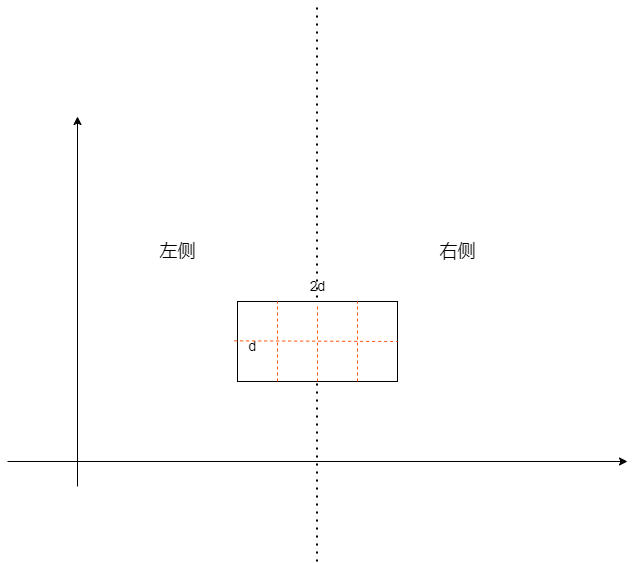
\includegraphics[width=0.4\linewidth]{asserts/最短点对问题.drawio.png}
    \caption{构造集合$C(\text{Loc}_i)$}
    \label{fig:enter-label}
\end{figure}

对于集合$C(\text{Loc}_i)$的构造,并不需要遍历$B$中所有的元素,考虑这么一个$x$方向长度为$2d$,$y$方向长度为$d$的长方形,将其对称分为如上图:



\subsection{算法与伪代码}

\begin{algorithm}[H]
\LinesNumbered
\caption{最近村庄距离问题}
\KwIn{一个正整数$n$,表示村庄数目,一个所有村庄位置数组$\text{Loc}$}
\KwOut{一个数$Ans$,表示这$n$个村庄中最近的两个村庄之间的距离}

\Function{$main(n,\text{Loc})$}{
    $\text{MergeSort}(\text{Loc}.x, 1, n)$ \Comment{使用题目二中的归并排序对\text{Loc}按照x坐标进行排序}\\
    \Return{$minDist(\text{Loc},1,n)$}
}

\Function{$minDist(\text{Loc},left, right)$}{
    \If{$right - left \le 3$}{
        $D\leftarrow \infty$\\
        \For{$i\leftarrow left\ to \ right-1$}{
            \For{$j \leftarrow i+1 \ to \ right$}{
                $D\leftarrow min(\sqrt{(\text{Loc}_i.x-\text{Loc}_j.x)^2 + (\text{Loc}_i.y-\text{Loc}_j.y)^2},D)$
            }
        }
        $\text{MergeSort}(\text{Loc}.y, left, right)$ \Comment{使用题目二中的归并排序对\text{Loc}按照y坐标进行排序}\\
        \Return{$D$}
    }
    $mid \leftarrow \frac{left+right}{2}$\\
    $D_1 \leftarrow minDist(\text{Loc},left, mid)$\\
    $D_2 \leftarrow minDist(\text{Loc},mid+1, right)$\\
    $D = mid(D_1, D_2)$\\
    $\text{Merge}(\text{Loc}.y, left, mid, right)$\Comment{使用题目二中的归并对\text{Loc}进行按照y坐标排序后的合并}\\
    $B\leftarrow CreateArray()$ \Comment{新建一个数组$B$}\\
    \For{$i\leftarrow left \ to \ right$}{
        \If{$|\text{Loc}_i.x - \text{Loc}_{mid}.x| < D$}{
            $B.add(\text{Loc}_i)$
        }
    }
    \For{$i \leftarrow 2 \ to \ B.length$}{
        \For{$j \leftarrow i-1 \ to\ max(0,i-7)$}{
            $D\leftarrow min(\sqrt{(\text{Loc}_i.x-\text{Loc}_j.x)^2 + (\text{Loc}_i.y-\text{Loc}_j.y)^2},D)$
        }
    }
    \Return{D}
}

\end{algorithm}

\subsection{时间复杂度分析}

该算法主要分为几个部分

\begin{enumerate}
    \item 最开始对数组进行按照$x$坐标进行归并排序,时间复杂度为$O(n\log n)$
    \item 使用分治法进行最短点对距离的求解
\end{enumerate}

第二次分治时,考虑有$T(n) = 2T(\frac{n}{2}) + f(n)$,其中$f(n)$表示合的过程的中的时间复杂度。

计算合并操作中更新跨数组最近点对的时间复杂度:

由于$C(\text{Loc}_i)$中的所有点的纵坐标都在$(y_i-h,y_i]$范围内;且$C(\text{Loc}_i)$中的所有点和$\text{Loc}_i$本身的横坐标都在$(x_m-d,x_m+d)$范围内。这构成了一个$2d\times d$的矩形。

根据$Figure1$所示,我们再将这个矩形拆分为两个$d\times d$的正方形,不考虑$\text{Loc}_i$,其中一个正方形中的点为$C(\text{Loc}_i)\cap A_1$,另一个为$C(\text{Loc}_i)\cap A_2$,由于它们来自同一下层递归,因此两个正方形内的任意两点间距离大于等于$d$。

接下来即可证明每个$d\times d$的正方形内最多有4个点:

将一个$d\times d$的正方形拆分为四个$\frac{d}{2}\times\frac{d}{2}$的小正方形。则每个小正方形中最多有$1$个点:因为该小正方形中任意两点最大距离是对角线的长度,即$\frac{d}{\sqrt 2}$,该数小于$d$。

根据\textbf{鸽巢原理},若有大于等于5个点,则必有两个点在同一个小正方形中,那么这两个小正方形之间的距离必然小于$d$,与两个正方形内的任意两点间距离大于等于$d$矛盾。由此,每个正方形中最多有$4$个点,矩形中最多有$8$个点,去掉$\text{Loc}_i$本身,$\max(C(\text{Loc}_i))=7$。

综上可知,合并操作中,更新跨数组最近点对的时间复杂度为$7$即$O(1)$。

\begin{enumerate}
    \item \text{Merge}操作的时间复杂度为$O(n)$
    \item 遍历构造数组B的时间复杂度为$O(n)$
    \item 最后二重循环遍历B中元素时,由于最多只有7个点,因此时间复杂度为$O(B.length)*O(7) = O(n)$
\end{enumerate}

因此整个合并操作的时间复杂度为$O(n)$。又根据分治算法的时间复杂度为:

\begin{align*}   
    &T(n) = 2T(\frac{n}{2}) + O(n)
\end{align*}

由主定理法知算法时间复杂度为$O(nlogn)$



\end{document}
